\documentclass[10pt]{beamer}

% Beamer style
%\usetheme[secheader]{Madrid}
% \usetheme{CambridgeUS}
\useoutertheme{infolines}
\usecolortheme[rgb={0.65,0.15,0.25}]{structure}
% \usefonttheme[onlymath]{serif}
\beamertemplatenavigationsymbolsempty
%\AtBeginSubsection

% Packages
%\usepackage[french]{babel}
\usepackage[latin1]{inputenc}
\usepackage{color}
\usepackage{xspace}
%\usepackage{dsfont, stmaryrd}
\usepackage{amsmath, amsfonts, amssymb}
\usepackage{epsfig}
\usepackage{url}
\usepackage{/home/robin/LATEX/Biblio/astats}
%\usepackage[all]{xy}
\usepackage{graphicx}

% Commands
\definecolor{darkred}{rgb}{0.65,0.15,0.25}
\newcommand{\emphase}[1]{\textcolor{darkred}{#1}}
% \newcommand{\emphase}[1]{{#1}}
\newcommand{\paragraph}[1]{\textcolor{darkred}{#1}}
\newcommand{\refer}[1]{{\footnotesize{\textcolor{gray}{[{\cite{#1}}]}}}}
\newcommand{\Refer}[1]{{\footnotesize{\textcolor{gray}{[{#1}]}}}}
\renewcommand{\newblock}{}

% Symbols
\newcommand{\Abf}{{\bf A}}
\newcommand{\Beta}{\text{B}}
\newcommand{\Bcal}{\mathcal{B}}
\newcommand{\BIC}{\text{BIC}}
\newcommand{\Ccal}{\mathcal{C}}
\newcommand{\dd}{\text{~d}}
\newcommand{\dbf}{{\bf d}}
\newcommand{\Dcal}{\mathcal{D}}
\newcommand{\Esp}{\mathbb{E}}
\newcommand{\Espt}{\widetilde{\Esp}}
\newcommand{\Ebf}{{\bf E}}
\newcommand{\Ecal}{\mathcal{E}}
\newcommand{\Gcal}{\mathcal{G}}
\newcommand{\Gam}{\mathcal{G}\text{am}}
\newcommand{\Hcal}{\mathcal{H}}
\newcommand{\Ibb}{\mathbb{I}}
\newcommand{\Ibf}{{\bf I}}
\newcommand{\ICL}{\text{ICL}}
\newcommand{\Cov}{\mathbb{C}\text{ov}}
\newcommand{\Corr}{\mathbb{C}\text{orr}}
\newcommand{\Var}{\mathbb{V}}
\newcommand{\Vsf}{\mathsf{V}}
\newcommand{\pen}{\text{pen}}
\newcommand{\pt}{\widetilde{p}}
\newcommand{\Fcal}{\mathcal{F}}
\newcommand{\Hbf}{{\bf H}}
\newcommand{\Jcal}{\mathcal{J}}
\newcommand{\Kbf}{{\bf K}}
\newcommand{\Lcal}{\mathcal{L}}
\newcommand{\Mcal}{\mathcal{M}}
\newcommand{\mbf}{{\bf m}}
\newcommand{\mum}{\mu(\mbf)}
\newcommand{\Ncal}{\mathcal{N}}
\newcommand{\Nbf}{{\bf N}}
\newcommand{\Nm}{N(\mbf)}
\newcommand{\Ocal}{\mathcal{O}}
\newcommand{\Obf}{{\bf 0}}
\newcommand{\Omegas}{\underset{s}{\Omega}}
\newcommand{\Pbf}{{\bf P}}
\newcommand{\Pt}{\widetilde{P}}
\newcommand{\Pcal}{\mathcal{P}}
\newcommand{\Qcal}{\mathcal{Q}}
\newcommand{\Rbb}{\mathbb{R}}
\newcommand{\Rcal}{\mathcal{R}}
\newcommand{\Scal}{\mathcal{S}}
\newcommand{\Ucal}{\mathcal{U}}
\newcommand{\Vcal}{\mathcal{V}}
\newcommand{\BP}{\text{BP}}
\newcommand{\EM}{\text{EM}}
\newcommand{\VEM}{\text{VEM}}
\newcommand{\VBEM}{\text{VBEM}}
\newcommand{\cst}{\text{cst}}
\newcommand{\obs}{\text{obs}}
\newcommand{\ra}{\emphase{\mathversion{bold}{$\rightarrow$}~}}
%\newcommand{\transp}{\text{{\tiny $\top$}}}
\newcommand{\transp}{\text{{\tiny \mathversion{bold}{$\top$}}}}
\newcommand{\logit}{\text{logit}\xspace}

% Directory
\newcommand{\figmixt}{/home/robin/ENSEIGN/COURS/MELANGE}
\newcommand{\figbma}{/home/robin/RECHERCHE/RUPTURES/MELANGE/Exemples/Grippe}
\newcommand{\fignet}{../FIGURES}
\newcommand{\figeco}{/home/robin/RECHERCHE/ECOLOGIE/EXPOSES/FIGURES}
%\newcommand{\figmotif}{/home/robin/RECHERCHE/RESEAUX/Motifs/FIGURES}


%====================================================================
%====================================================================

%====================================================================
%====================================================================
\begin{document}
%====================================================================
%====================================================================

%====================================================================
\title[GOF for graph models]{Goodness of fit of logistic models for random graphs: \\
a variational Bayes approach}

\author[S. Robin]{S. Robin \\ ~\\
  Joint work with P. Latouche and S. Ouadah}

\institute[INRA / AgroParisTech]{INRA / AgroParisTech \\ ~\\
  \vspace{-.1\textwidth}
  \begin{tabular}{ccccc}
%     
\includegraphics[height=.3\textheight]{\fignet/LogoINRA-Couleur} & 
%     \hspace{.02\textheight} &
%     
\includegraphics[height=.08\textheight]{\fignet/logagroptechsolo} & 
%     \hspace{.02\textheight} &
%     
\includegraphics[height=.09\textheight]{\fignet/logo-ssb}
    
\includegraphics[height=.2\textheight]{\fignet/LogoINRA-Couleur} & 
    \hspace{.02\textheight} &
    
\includegraphics[height=.067\textheight]{\fignet/logagroptechsolo} & 
    \hspace{.02\textheight} &
    
\includegraphics[height=.06\textheight]{\fignet/logo-ssb}
    \\ 
  \end{tabular} \\
  \bigskip
  }

\date[May 2016, Montpellier]{JdS - SFB, May 2016, Montpellier}

%====================================================================
%====================================================================
\maketitle
%====================================================================

%====================================================================
%====================================================================
\section*{Problem}
%====================================================================
\frame{ \frametitle{Problem}

  \paragraph{Ecological network} $Y = (Y_{ij})_{1 \leq i, j \leq n}$: interactions between $n$ tree species:
  $$
  Y_{ij} = \Ibb\{i \sim j\}  = \Ibb\{\text{$i$ and $j$ share some fungal parasite}\}
  $$
  
  \bigskip \bigskip \pause
  \paragraph{+ Covariates} $x = (x_{ij})_{1 \leq i, j \leq n}$:
  \begin{itemize}
   \item $x^1_{ij}$ = phylogenetic distance between $i$ and $j$,
   \item $x^2_{ij}$ = geographic distance between the typical habitat of $i$ and $j$,
   \item ...
  \end{itemize}

  \bigskip \bigskip \pause
  \begin{overprint}
   \onslide<3>
  \paragraph{Questions:} 
  \begin{itemize}
   \item Can we explain the topology of $Y$ based on $x$? 
   \item Is there a residual heterogeneity in the network $Y$? 
  \end{itemize}
   \onslide<4>
  \paragraph{Questions:} 
  \begin{itemize}
   \item Can we explain the topology of $Y$ based on $x$? \qquad \ \ \emphase{\ra logistic regression}
   \item Is there a residual heterogeneity in the network $Y$? \quad \emphase{\ra $W$-graph}
  \end{itemize}
  \end{overprint}
  }
  
%====================================================================
\frame{\frametitle{Outline} \tableofcontents}

% %====================================================================
% %====================================================================
% \section{Variational Bayes inference}
% \frame{\frametitle{Outline} \tableofcontents[currentsection]}

%====================================================================
%====================================================================
\section{Reminder of variational Bayes inference}
\frame{\frametitle{Outline} \tableofcontents[currentsection]}
%====================================================================
\frame{\frametitle{Variational (Bayes) inference}

  \bigskip
  $Y=$ observed data, $Z=$ latent variable, $\theta=$ parameter. 
  
  \bigskip
  Frequentist and Bayesian inference often requires
  $$
  p(Z|Y), \qquad p(\theta|Y) \quad \text{or} \quad p(\theta, Z|Y).
  $$
  
  \pause \bigskip \bigskip
  \paragraph{Variational inference:} find
  $
  q(\cdot) \approx p(\cdot|Y).
  $
  
  \pause \bigskip \bigskip 
  Typically \refer{Jaa00,Min05,WaJ08}
  $$
  q^* = \arg\min_{q \in \Qcal} D[\pt(\cdot) || p(\cdot|Y)]
  $$
  \begin{tabular}{cc}
   \begin{tabular}{p{.45\textwidth}}
   \vspace{-.05\textheight}
    \begin{itemize}
    \item $D[q||p] = KL[q||p]$; 
    \item $\pt(\theta) = \Ncal$;
    \end{itemize}
   \end{tabular}
   &
   \begin{tabular}{p{.45\textwidth}}
   \vspace{-.05\textheight}
    \begin{itemize}
    \item $\pt(Z) = \prod_i q_i(Z_i)$;
    \item $\pt(\theta, Z) = \pt(\theta) \pt(Z)$.
    \end{itemize}
   \end{tabular}
  \end{tabular}


}

%====================================================================
\frame{\frametitle{Variational Bayes EM (VBEM)}

  \bigskip
  \paragraph{Aim:} \refer{BeG03}
  $$
  \min_{\pt} KL[\pt(\theta) \textcolor{red}{\times} \pt(Z) || p(\theta, Z|Y)].
  $$

  \bigskip \pause
  \paragraph{Algorithm.} 'mean-field' principle:
  \begin{eqnarray*}
    \text{VE-step:} \qquad \pt^{(h+1)}(Z) & \propto & \exp \left[\Esp_{\pt^{(h)}(\theta)} \log p(\theta, Z ,Y) \right] \\
    \text{VM-step:} \qquad \pt^{(h+1)}(\theta) & \propto & \exp \left[\Esp_{\pt^{(h+1)}(Z)} \log p(\theta, Z ,Y) \right] 
  \end{eqnarray*}
  + close-form update formulas in the conjugate prior-exponential family setting.

  \bigskip \bigskip \pause
  \paragraph{By-product:} same probem as
  $$
  \max_{\pt} \ \log p(Y) - KL[\pt(\cdot, \cdot) || p(\cdot, \cdot|Y)] 
  $$
  \ra computable lower bound of $\log p(Y)$: $\Espt[\log p(\theta, Z, Y)] - \Espt[\log \pt(\theta, Z)]$.

}

%====================================================================
%====================================================================
\section{Accounting for covariates}
\frame{\frametitle{Outline} \tableofcontents[currentsection]}
%====================================================================
\frame{\frametitle{Logistic regression}

  \paragraph{Forget about the network structure:} $(Y_{ij})$ are independent
  $$
  Y_{ij} \sim \Bcal[g(x_{ij}^\intercal \beta)], 
  \qquad
  g(u) = e^u / (1 + e^u)
  $$
  
  \bigskip \bigskip \pause
  \paragraph{Bayesian inference.} Prior on $\beta$:
  $$
  \beta \sim \Ncal(0, \eta^{-1} I)
  $$
  
  \bigskip
  {Posterior distribution:} 
  $$
  p(\beta|Y) \propto p(\beta) p(Y|\beta)
  $$
  \ra No nice conjugacy hold for the normal prior / logistic regression model \\
  \ra No close form for the posterior $p(\beta | Y)$.
  

  }
  
%====================================================================
\frame{\frametitle{Variational Bayes inference}

  \begin{tabular}{ll}
    \hspace{-.05\textwidth}
    \begin{tabular}{p{.5\textwidth}}
    Nasty term in $\log p(Y | \beta)$:
    $$
    -\log (1 + e^{-x_{ij} \beta}).
    $$
    
    \pause \bigskip
    \refer{JaJ00}: quadratic lower bound of $\log p(\beta, Y)$ to get 
    $$
    p(\beta|Y) \approx \pt(\beta) = \Ncal(\beta; \mu_\beta, S_\beta).
    $$
    \end{tabular}
    & 
    \hspace{-.05\textwidth}
    \begin{tabular}{p{.5\textwidth}}
      \includegraphics[width=.45\textwidth]{../FIGURES/ApproxJaJ00}
    \end{tabular}
  \end{tabular}

%   
%   \pause \bigskip
%   \refer{JaJ00} observe that 
%   $$
%   -\log (1 + e^{-u}) = \frac{u}2 - \log(e^{u/2} + e^{-u/2})
%   $$ 
%   where $- \log(e^{u/2} + e^{-u/2})$ is convex in $u^2$, so a quadratic lower bounding of $\log p(\beta, Y)$ can be derived to get 
%   $$
%   p(\beta|Y) \approx \pt(\beta) = \Ncal(\beta; \mu_\beta, S_\beta).
%   $$
  
  \pause
  \paragraph{Example: Tree network.} $n = 51$ tree species, ($N = 1275$ pairs), 3 distances:
  $$
  \begin{array}{rrrrr}
   & \text{intercept} & \text{genetic} & \text{geographic} & \text{taxonomic} \\
   \hline
   \mu_{\beta} & 0.221 & 0.060 & -0.337 & -0.811 \\
   \sigma_{\beta} & 0.058 & 0.062 & 0.059 & 0.060 \\
  \end{array}
  $$

}

%====================================================================
%====================================================================
\section{Heterogeneous network models}
\frame{\frametitle{Outline} \tableofcontents[currentsection]}
%====================================================================
\frame{\frametitle{Latent space models}

  Most observed networks are heterogeneous in terms of degree distribution, node centrality, existence of clusters, ...
  
  \bigskip \bigskip \pause
  \paragraph{Generic framework \refer{BJR07}:}
  \begin{itemize}
   \item Latent variable for node $i$: $Z_i \sim \pi$.
   \item Edges $Y_{ij}$ conditionally independent: 
  \end{itemize}
  $$
  (Z_i) \text{ iid } \sim \pi, 
  \qquad 
  Y_{ij} \ | \ (Z_i): Y_{ij} \sim \Bcal[\emphase{\gamma(Z_i, Z_j)}]
  $$ 
  
  \bigskip \pause
  Includes \Refer{Matias and R. (2014)}\nocite{MaR14}: 
  \begin{itemize}
   \item stochastic block-model \refer{FrH82}, 
   \item latent position models \refer{HRH02,HRT07,DPV10}, 
   \item $W$-graph \refer{LoS06,DiJ08}.
  \end{itemize}
  }

%====================================================================
\frame{ \frametitle{Variational Bayes for heterogeneous network models}

  \begin{tabular}{cc}
    \hspace{-.05\textwidth}
    \begin{tabular}{p{.5\textwidth}}
      \onslide+<1->{
        \paragraph{Graphical model} formalism \\
        \refer{Lau96}. \\ ~\\ }
        \onslide+<2->{\paragraph{'Frequentist' setting ($p(\cdot|\theta)$):}}
        \begin{itemize}
        \onslide+<2->{\item iid $Z_i$'s,}
        \onslide+<3->{\item $p(Y_{ij} | Z_i, Z_j)$,}
        \onslide+<4->{\item $p(Z_i, Z_j|Y)$: graph moralization,}
        \onslide+<5->{\item this holds for each pair $(i, j)$,}
        \end{itemize}
    \end{tabular}
    & 
    \hspace{-.02\textwidth}
    \begin{tabular}{p{.5\textwidth}}
	 \begin{overprint}
        \onslide<2>
        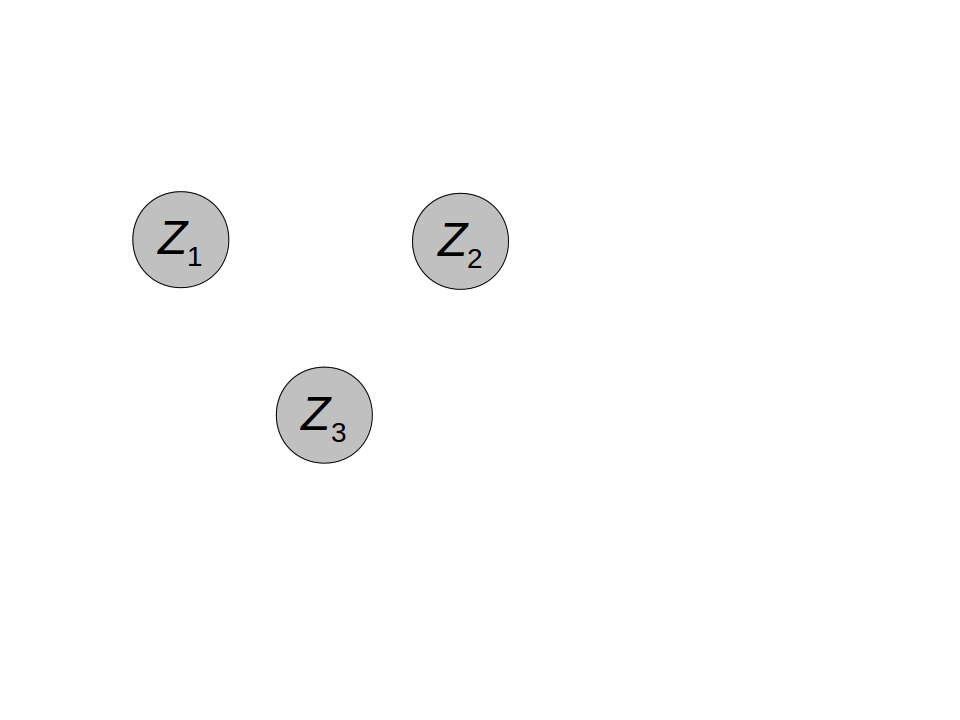
\includegraphics[width=0.6\textwidth]{../FIGURES/FigSBM-Z}
        \onslide<3>
        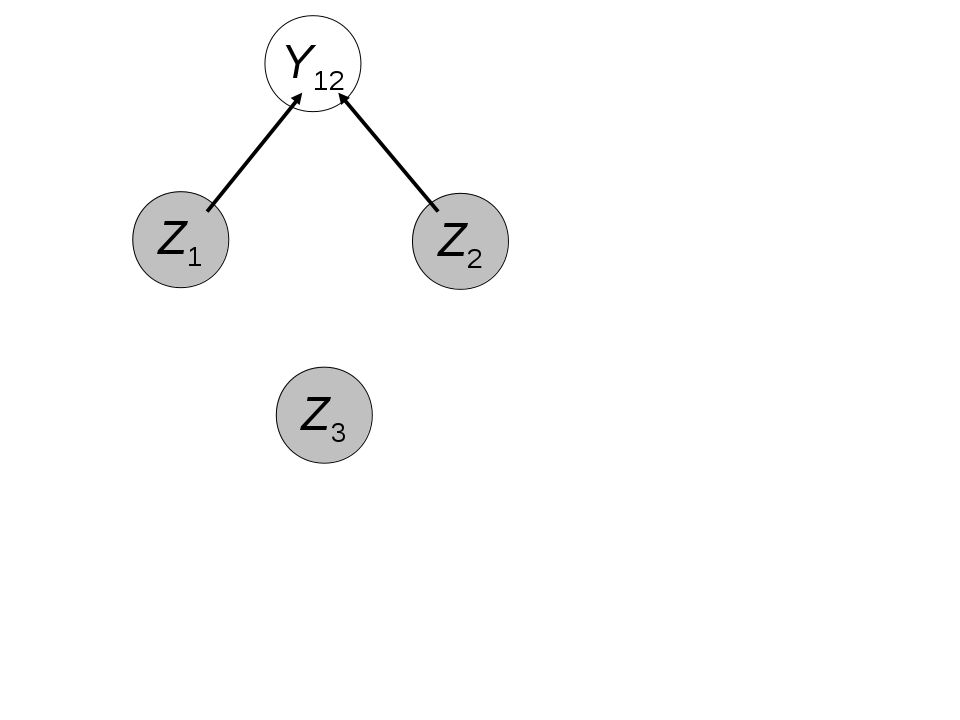
\includegraphics[width=0.6\textwidth]{../FIGURES/FigSBM-Z-Y12}
        \onslide<4>
        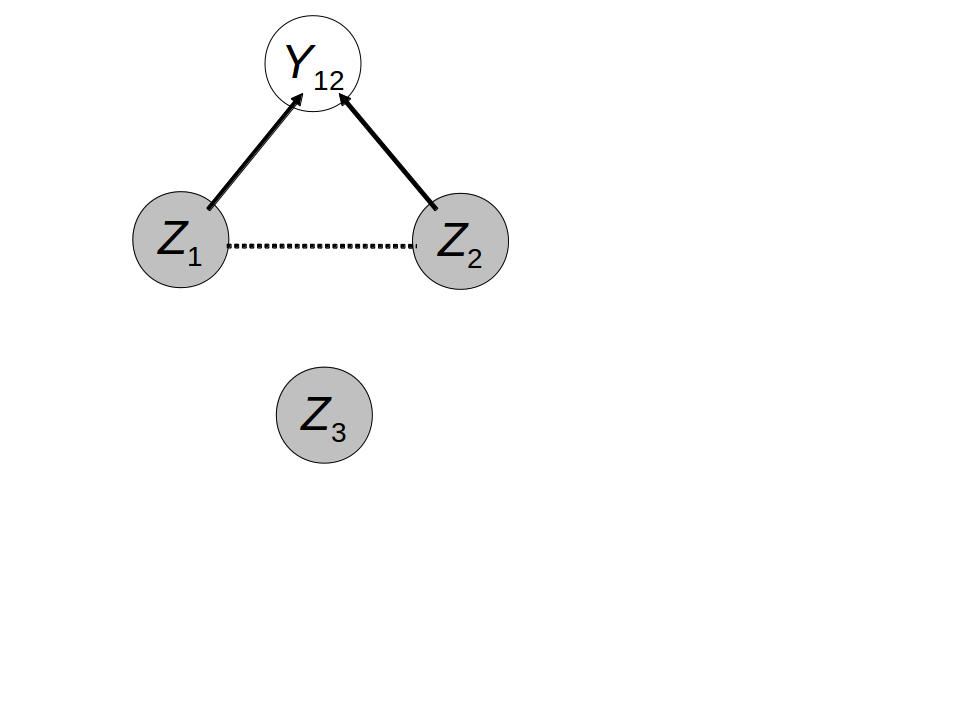
\includegraphics[width=0.6\textwidth]{../FIGURES/FigSBM-Z-Y12-Moral} 
        \onslide<5>
        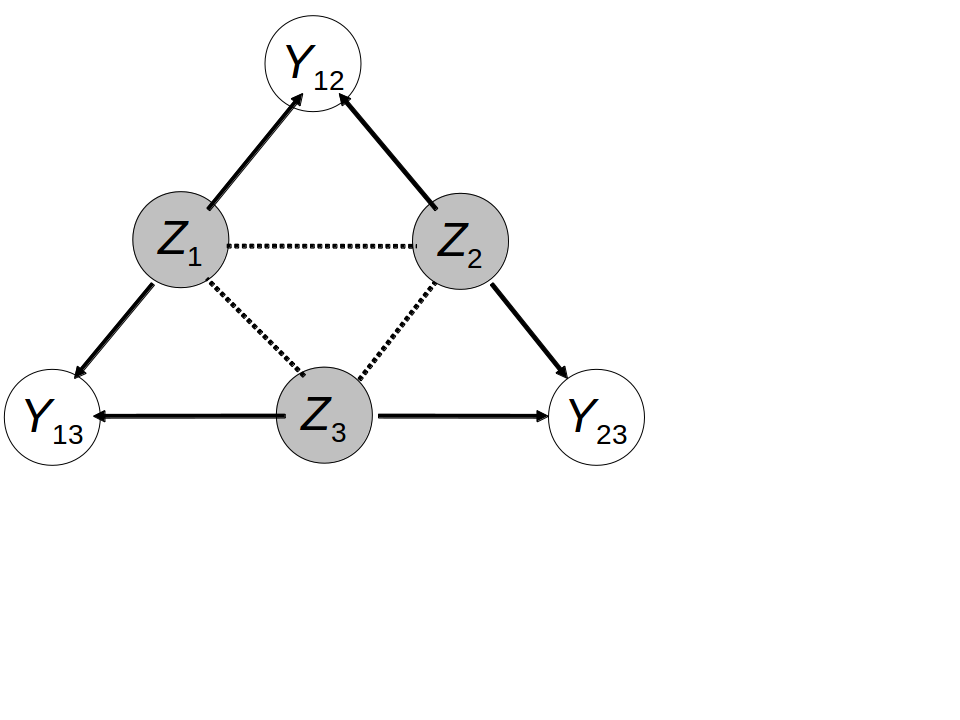
\includegraphics[width=0.6\textwidth]{../FIGURES/FigSBM-Z-Y-Moral} 
        \onslide<6>
        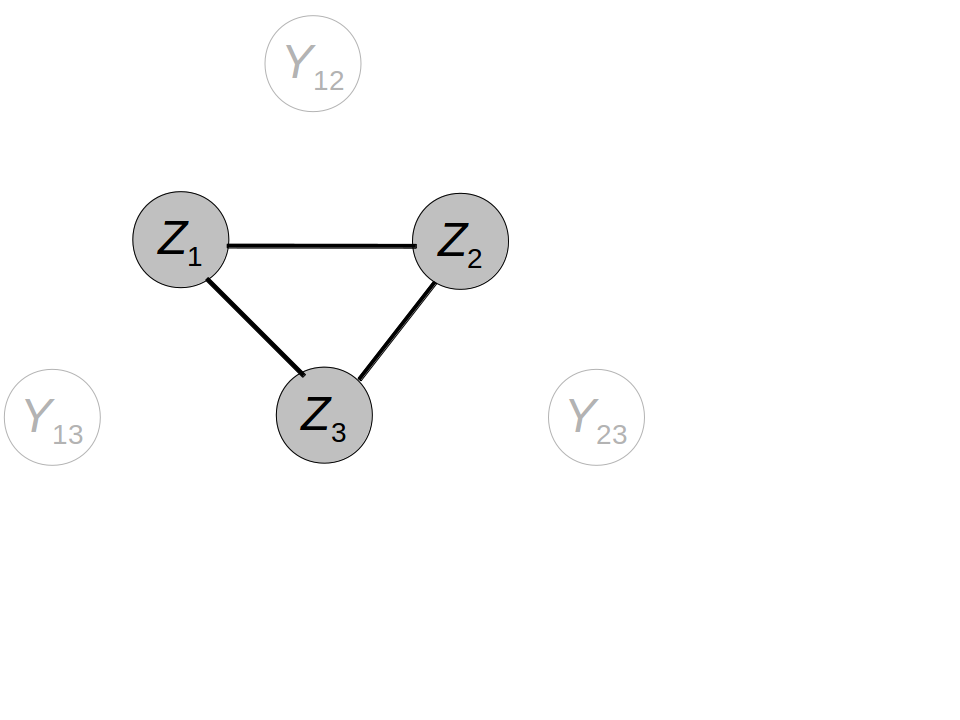
\includegraphics[width=0.6\textwidth]{../FIGURES/FigSBM-ZcondY}
        \onslide<7->
        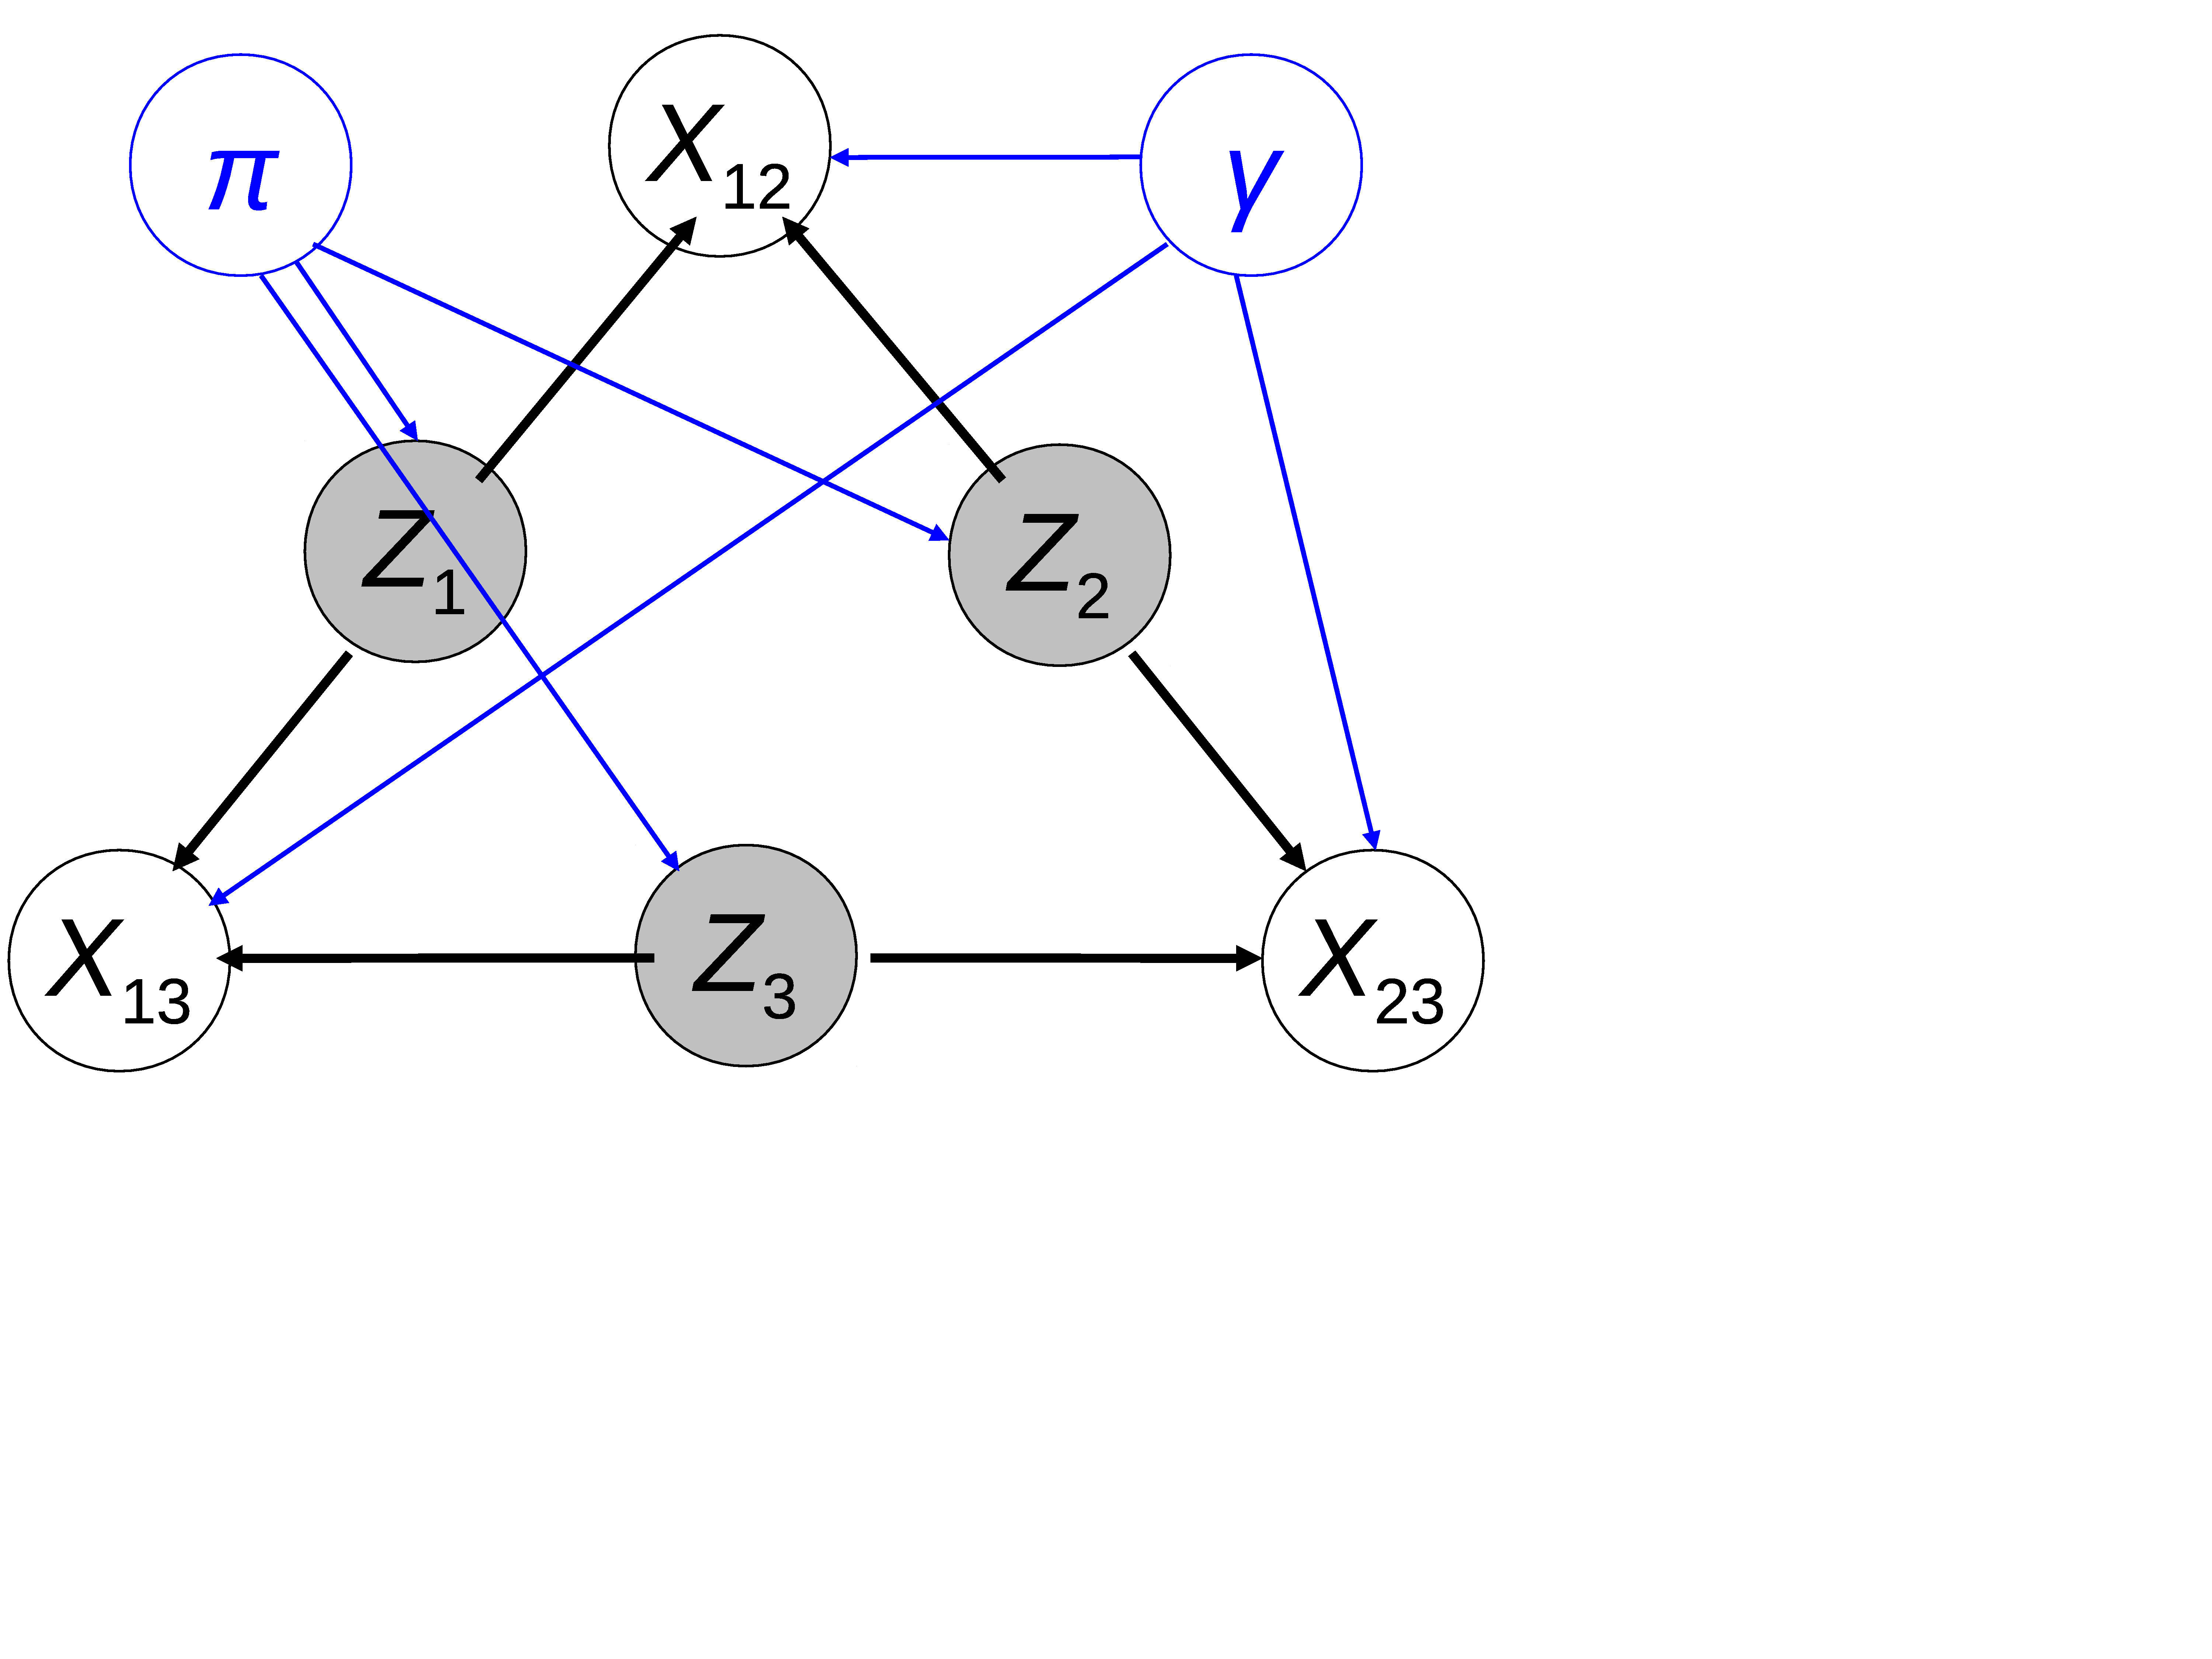
\includegraphics[width=0.6\textwidth]{../FIGURES/FigSBM-Bayes}
      \end{overprint}
    \end{tabular}
  \end{tabular}

  \vspace{-.05\textheight}
  \onslide<6->{
  \paragraph{Dependency graph of $p(Z|Y, \theta) =$ clique.}  \\
  \ra No factorization can be hoped (unlike for HMM). \\
  \ra $p(Z | Y, \theta)$ can not be computed (efficiently). \\ }
  \onslide<7>{
  \paragraph{Bayesian setting.} Things get worst.}

}

%====================================================================
\frame{ \frametitle{$W$-graph (graphon)  model}

  \begin{tabular}{cc}
    \hspace{-.02\textwidth}
    \begin{tabular}{p{.5\textwidth}}
	 Latent variables:
	 $$
	 (U_i) \text{ iid } \sim \Ucal_{[0, 1]},
	 $$ ~\\
	 \emphase{Graphon} function $\gamma$:
	 $$
	 \gamma(u, u'): [0, 1]^2 \rightarrow [0, 1]
	 $$ ~\\    
	 Edges:
	 $$
	 P(Y_{ij} = 1|U_i, U_j) = \gamma(U_i, U_j)
	 $$    
	 \end{tabular}
    & 
    \hspace{-.1\textwidth}
    \begin{tabular}{p{.5\textwidth}}
	 Graphon function $\gamma(u, u')$ \\
      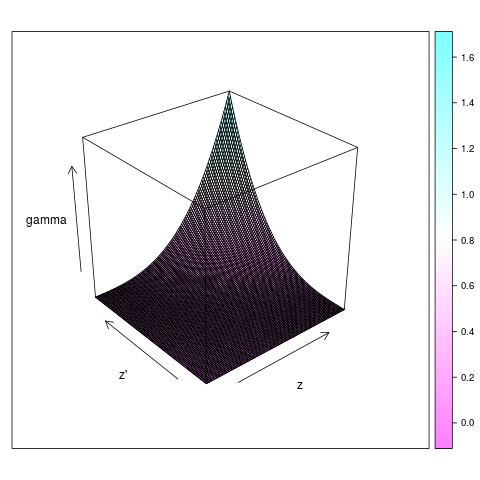
\includegraphics[width=.5\textwidth]{../FIGURES/FigCLADAG-W-graphon} \\
    \end{tabular}
  \end{tabular}
  
 }

%====================================================================
\frame{\frametitle{Some typical graphon functions}

  Graphon function $\gamma$: a global picture of the network's topology.

  \bigskip \bigskip 
  \centerline{
  \begin{tabular}{ccc}
  'Scale free' & Community & Small world \\
  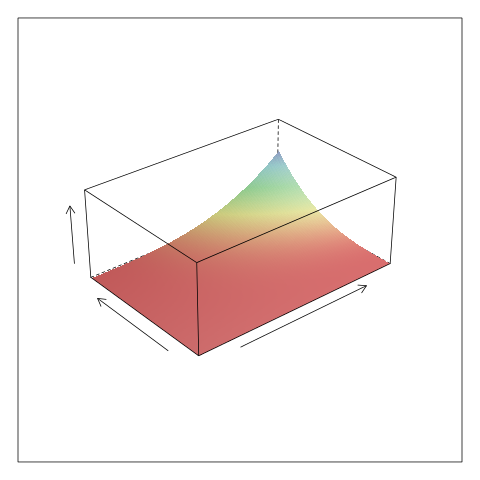
\includegraphics[width=.3\textwidth]{../FIGURES/EDD-ScaleFreeTrueGraphon} &
  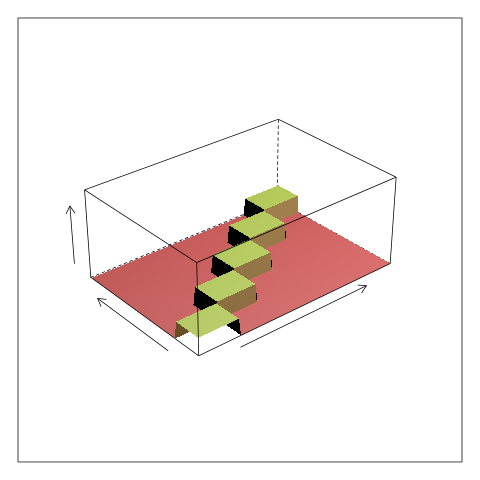
\includegraphics[width=.3\textwidth]{../FIGURES/CommunityTrueGraphon} &
  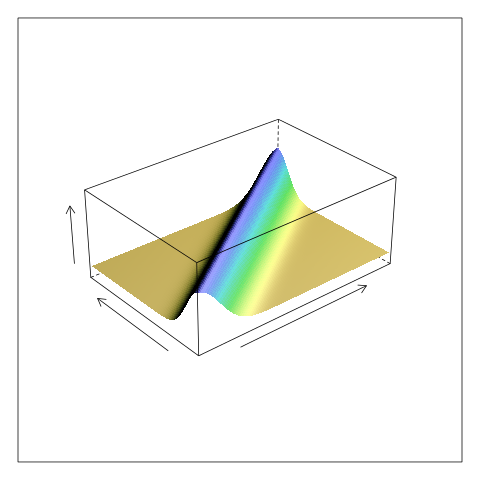
\includegraphics[width=.3\textwidth]{../FIGURES/SmallWorldTrueGraphon} 
  \end{tabular}
  } 
  
  \bigskip \pause
  \paragraph{Remark:} $\gamma(\cdot, \cdot) = $cst \ra ER model
  
}

%====================================================================
\frame{ \frametitle{Variational Bayes inference of the graphon (1/3)}

  \paragraph{Stochastic Block-model (SBM) as a $W$-graph model.} 

  \bigskip
  \begin{tabular}{cc}
    \hspace{-.02\textwidth}
    \begin{tabular}{p{.5\textwidth}}
	 Latent variables:
	 $$
	 (Z_i) \text{ iid } \sim \Mcal(1, \pi)
	 $$
	 Blockwise constant graphon:
	 $$
	 \gamma(z, z') = \gamma_{k\ell}
	 $$
	 Edges:
	 \begin{eqnarray*}
	 P(Y_{ij} = 1|Z_i, Z_j) & = & \gamma(Z_i, Z_j) \\
	 \logit (~"~) & = & Z_i^\intercal \alpha Z_j \\
	 \alpha & = & \logit(\gamma)
	 \end{eqnarray*}    
	 \end{tabular}
    & 
    \hspace{-.1\textwidth} \pause
    \begin{tabular}{p{.5\textwidth}}
	 Graphon function $\gamma^{SBM}_K(u, u')$ \\
      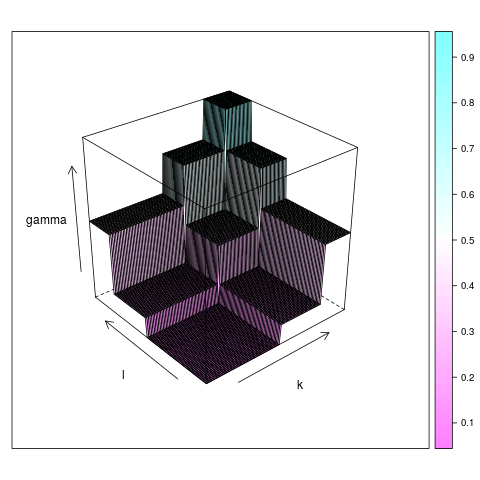
\includegraphics[width=.45\textwidth]{../FIGURES/FigCLADAG-SBM-graphon} \\
    \end{tabular}
  \end{tabular} 

  \ra block widths $= \pi_k$, block heights $\gamma_{k\ell}$
 }

%====================================================================
\frame{ \frametitle{Variational Bayes inference of the graphon (2/3)}

  \begin{tabular}{cc}
    \hspace{-.02\textwidth}
    \begin{tabular}{p{.45\textwidth}}
    \paragraph{VBEM for SBM:} conjugate prior-exponential family setting \\
    \refer{LBA12}.
    
    \bigskip \bigskip \pause
    Approximate posteriors
    \begin{eqnarray*}
    \pt(\pi) & = & \Dcal(\widetilde{\pi}) \\
    \pt(\gamma_{k\ell}) & = & \Beta(\widetilde{\gamma}^0_{k\ell}, \widetilde{\gamma}^1_{k\ell}) \\
    \pt(Z_i) & = & \Mcal(1; \widetilde{\tau}_i) \\
    \end{eqnarray*}
 
%     \bigskip \pause
%     \paragraph{Estimate of $\gamma(u, v)$.} 
%     Due \\
%     to the uncertainty of the $\pi_k$, \\
%     the posterior mean of $\gamma^{SBM}_K$  \\
%     is smooth
%     
%     \bigskip 
%     (Explicit integration using \refer{GoS10})
    \end{tabular}
    & 
    \hspace{-.05\textwidth} \pause
    \begin{tabular}{p{.5\textwidth}}
	 Posterior mean $\Espt[\gamma^{SBM}_K(u, u')]$ \\
      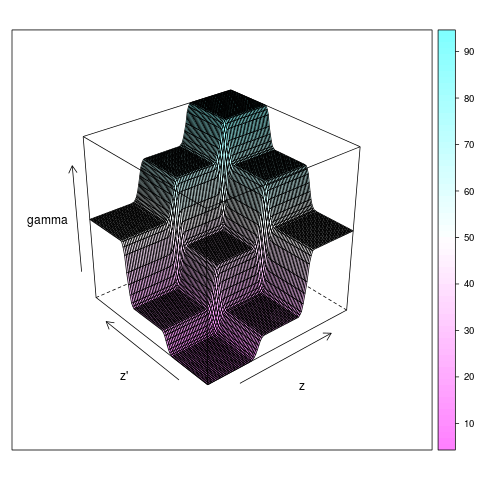
\includegraphics[width=.45\textwidth]{../FIGURES/FigGraphon-SBM-average} \\
    \end{tabular}
  \end{tabular}
  
}

%====================================================================
\frame{ \frametitle{Variational Bayes inference of the graphon (3/3)}

%   The graphon model does not rely on any true $K$.

  \bigskip
  \paragraph{Bayesian model averaging (BMA):} Fit SBM with $K = 1, \dots K_{\max}$ and compute
  $$
  \Esp[\gamma(u, u') | Y] = \sum_{K \geq 1} \emphase{p(K|Y)} ~ \Esp[\gamma_K^{SBM}(u, u') | Y]
  $$

%   \bigskip \pause
%   \paragraph{Pushing the variational approximation further:} Consider the model $K$ as an additional hidden variable:
%   $$
%   p(Z, \theta, K|Y) \approx \pt(Z, \theta, K) 
%   := \pt(Z|K) \times \pt(\theta|K) \times \pt(K)  
%   $$
%   
  \bigskip \bigskip \pause
  \paragraph{Variational approximation of $p(K|Y)$ \refer{VMR12}.}
  $$
  \pt(K) \propto p(K) ~ e^{\log p(Y|K) - KL(K)} = p(K|Y)~ e^{-\emphase{KL(K)}}
  $$ 
  where $KL(K) =$ minimized $KL$ divergence with $K$ groups. 
  
  \bigskip \bigskip \bigskip \pause
  \paragraph{VBMA estimate of the graphon \Refer{Latouche and R. (2015)}\nocite{LaR15}:}
  $$
  \Espt[\gamma(u, u')] = \sum_K \emphase{\pt(K)} ~ \Espt[\gamma_K^{SBM}(u, u')].
  $$

}

%====================================================================
\frame{\frametitle{Example: Tree network}

  $n = 51$ tree species. Inferred graphon function:
  $$
  \includegraphics[height=.5\textheight]{../FIGURES/treed0} 
  $$
  }

%====================================================================
\frame{\frametitle{Example: Political blog network}

  $n = 196$ blogs. Inferred graphon function:
  $$
  \includegraphics[height=.5\textheight]{../FIGURES/blogd0} 
  $$
  
  \pause
  \begin{itemize}
   \item Graphical representation of the network.
   \item Interpretability...
  \end{itemize}
  }

%====================================================================
%====================================================================
\section{Goodness-of-fit}
\frame{\frametitle{Outline} \tableofcontents[currentsection]}
%====================================================================
\frame{\frametitle{Original problem}

  \paragraph{Data:}
  \begin{itemize}
   \item $Y =$ observed (binary) network
   \item $x = $ covariates
  \end{itemize}

  \bigskip \bigskip 
  \paragraph{Questions:}
  \begin{itemize}
   \item Does $x$ explain the topology of $Y$?
   \item Residual (wrt $x$) heterogeneity in $Y$?
  \end{itemize}

}

%====================================================================
\frame{\frametitle{Combined model}

  \bigskip
  \paragraph{Logistic regression:}
  $$
  \logit~P(Y_{ij} = 1) = 
  \textcolor{red}{\beta_0} + \sum_k \beta_k x_{ij}^k
  $$

  \bigskip \bigskip \pause
  \paragraph{Logistic regression + graphon residual term:} $(U_i)$ iid $\sim \Ucal[0, 1]$,
  $$
  \logit~P(Y_{ij} = 1 |U_i, U_j) = 
  \textcolor{red}{\phi(U_i, U_j)} + \sum_k \beta_k x_{ij}^k
  $$

  \bigskip \bigskip \pause
  \paragraph{Goodness of fit:} Check if
  $$
  \phi(u, u') = \cst \qquad (= \beta_0)
  $$
  }

%====================================================================
\frame{\frametitle{Goodness-of-fit as model comparison}

  \bigskip
  \paragraph{Auxiliary model $M_K$:} % $Z_i \sim \Mcal_K(1; \pi)$, $\alpha: K \times K$,
  $$
  \logit~P(Y_{ij} = 1 | U_i, U_j) = \textcolor{red}{\phi_K^{SBM}(U_i, U_j)} + \sum_k \beta_k x_{ij}^k.
  $$
%   \emphase{Model $M_K =$} logistic regression + $K$-class SBM residual. 
  
  \pause \bigskip \bigskip
  \paragraph{Model averaging} yields
  $$
  p(\phi | Y) = \sum_k p(K|Y) \ p(\phi_K^{SBM} | Y)
  $$

  \bigskip \pause
  \paragraph{Goodness of fit:} 
  $$
  \begin{array}{rclcl}
   H_0 & = & \{\text{logistic regression is sufficient}\} & = & M_1 \\
   H_1 & = & \{\text{logistic regression is not sufficient}\} & = & \bigcup_{K > 1} M_K 
  \end{array}
  $$
  GOF is a assessed if
  $$
  p(H_0|Y) = p(M_1|Y) \text{ is large.}
  $$

  }

%====================================================================
\frame{\frametitle{Variational Bayes inference}

  \bigskip
  \paragraph{VBEM:} A global variational Bayes EM algorithm can be designed to obtain all needed (approximate) posteriors:
  \begin{eqnarray*}
   p(\theta, Z, K|Y) & \approx & \pt(\theta, Z, K) 
   \quad = \quad \pt(K) \; \pt(\theta |K) \; \textcolor{red}{\times} \; \pt(Z | K) \\
   & = & \pt(K) \; \left(\pt(\alpha |K) \; \pt(\beta |K) \; \pt(\pi |K)\right) \; \textcolor{red}{\times} \; \left(\textcolor{red}{\prod_i} \; \pt(Z_i | K)\right)
  \end{eqnarray*}
%   $$
%   \pt(\beta|K), \qquad \pt(\pi|K), \qquad \pt(\alpha|K), \qquad \pt(Z|K), \qquad \pt(K).
%   $$
  
  \bigskip \pause
  \paragraph{Posterior quantities of interest:}
  \begin{itemize}
   \item Goodness of fit criterion:
   $$
   p(H_0|Y) \approx \Pt(K=1)
   $$
   \item Residual graphon:
   $$
   \widehat{\phi}(u, u') = \sum_K \pt(K) ~ \Espt[\phi^{SBM}_K(u, u')]
   $$
  \end{itemize}
  }

%====================================================================
%====================================================================
\section{Illustrations}
\frame{\frametitle{Outline} \tableofcontents[currentsection]}
%====================================================================
\frame{\frametitle{Political blog network}

  $n = 196$ blogs ($N = 19110$ pairs), 3 covariates, density $= .07$ 

  \bigskip
  \begin{tabular}{cc}
    \begin{tabular}{p{.5\textwidth}}
	 Inferred graphon (no covariate) \\ ~\\
	 \includegraphics[height=.4\textheight]{../FIGURES/blogd0} \\ ~\\
	 ~
    \end{tabular}
    & 
    \hspace{-.05\textwidth}
    \begin{tabular}{p{.5\textwidth}}
	 Residual graphon (3 covariates) \\ ~\\
	 \includegraphics[height=.4\textheight]{../FIGURES/blogd3} \\ ~\\
	 $\Pt(H_0) \simeq 10^{-172}$
    \end{tabular}
  \end{tabular}
  }

%====================================================================
\frame{\frametitle{Tree network}

  $n = 51$ species ($N = 1275$ pairs), 3 covariates, density $= .54$ 

  \bigskip
  \begin{tabular}{cc}
    \begin{tabular}{p{.5\textwidth}}
	 Inferred graphon (no covariate) \\ ~\\
	 \includegraphics[height=.4\textheight]{../FIGURES/treed0} \\ ~\\
	 ~
    \end{tabular}
    & 
    \hspace{-.05\textwidth}
    \begin{tabular}{p{.5\textwidth}}
	 Residual graphon (3 covariates) \\ ~\\
	 \includegraphics[height=.4\textheight]{../FIGURES/treed3} \\ ~\\
	 $\Pt(H_0) \simeq 10^{-152}$
    \end{tabular}
  \end{tabular}
  }

%====================================================================
\frame{\frametitle{Florentine business}

  $n = 16$ families ($N = 120$ pairs), 3 covariates, density $= .12$ 

  \bigskip
  \begin{tabular}{cc}
    \begin{tabular}{p{.5\textwidth}}
	 Inferred graphon (no covariate) \\ ~\\
	 \includegraphics[height=.4\textheight]{../FIGURES/businessd0} \\ ~\\
	 ~
    \end{tabular}
    & 
    \hspace{-.05\textwidth}
    \begin{tabular}{p{.5\textwidth}}
	 Residual graphon (3 covariates) \\ ~\\
	 \includegraphics[height=.4\textheight]{../FIGURES/businessd3} \\ ~\\
	 $\Pt(H_0) = .99$
    \end{tabular}
  \end{tabular}
  }

%====================================================================
%====================================================================
\section*{Discussion}
% \frame{\frametitle{Outline} \tableofcontents[currentsection]}
%====================================================================
\frame{\frametitle{Discussion}

  \paragraph{Contribution:}
  \begin{itemize}
   \item Generic logistic regression model with a network residual term.
   \item Detour through SBM provides a natural goodness-of-fit criterion.
  \end{itemize}

  \bigskip \bigskip \pause
  \paragraph{Comments:}
  \begin{itemize}
   \item Strongly relies on variational Bayes approximation of the posteriors. 
   \item VBEM accurate for logistic regression and SBM separately.
   \item No clue about accuracy in the combined model.
   \end{itemize}

  \bigskip \bigskip \pause
  \paragraph{On-going work:}
  \begin{itemize}
   \item Sequential importance sampling: move from $\pt(\cdot)$ to $p(\cdot|Y)$ using a tempering scheme.
   \item and \dots
   \end{itemize}
}

%====================================================================
\frame{\frametitle{Cartable meeting: Toulouse, October 12-14}

  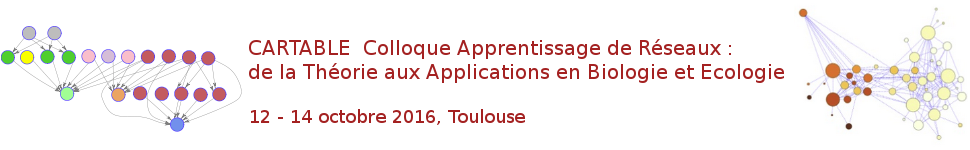
\includegraphics[width=\textwidth]{../FIGURES/Cartable-2016}
  
  \bigskip \bigskip
  \paragraph{Aim:} Bring together
  \begin{itemize}
   \item biologists
   \item ecologists
   \item computer scientists
   \item statisticians
  \end{itemize}
  involved in molecular and ecological network learning:
  
  $$
  \text{\textcolor{blue}{\tt https://cartable.sciencesconf.org/}}
  $$
  
}
%====================================================================
%====================================================================
\frame[allowframebreaks]{ \frametitle{References}
{\footnotesize
  \bibliography{/home/robin/Biblio/ARC,/home/robin/Biblio/BibGene}
  \bibliographystyle{/home/robin/LATEX/Biblio/astats}
%   \bibliographystyle{plain}
  }
}

%====================================================================
%====================================================================
\end{document}
%====================================================================
%====================================================================

  \begin{tabular}{cc}
    \begin{tabular}{p{.5\textwidth}}
    \end{tabular}
    & 
    \hspace{-.02\textwidth}
    \begin{tabular}{p{.5\textwidth}}
    \end{tabular}
  \end{tabular}

